\documentclass[a4paper,12pt]{article}
\usepackage[english]{babel}
\author{Steven Hill}
\title{Four Page Sample}
\date{\today}


\usepackage{rotating}
\usepackage{indentfirst}
\usepackage{lineno}
\usepackage{fancyhdr}
\pagestyle{fancy}
\usepackage[utf8]{inputenc}
\usepackage{amsmath}
\usepackage{amsfonts}
\usepackage{amssymb}
\usepackage{graphicx}
\usepackage{setspace}
\usepackage{outline}
\usepackage{paralist}


\newcommand{\bibent}{\noindent \hangindent 40pt}
\newenvironment{workscited}{ \doublespacing \newpage \begin{center} Works Cited \end{center}}{\newpage }

\begin{document}
\maketitle
\section{Introduction}
 Easy-Terminal-Alternative (ETA) is a web driven tool for interacting with command line applications. This document contains the background and technical documentation for the Easy-Terminal-Alternative implementation at the Center for Genome Research (CGRB) and Biocomputing. ETA's primary purpose is to assist researchers with using otherwise complicated computational tools in an easy, web-driven format.
 
 The biggest flaw with ETA to date is the lack of documentation. According to Carla Schroder, author of the 
Linux cookbook, "Good documentation is equally important as good code. Sometimes there is this attitude that developer time is more valuable and important than user or potential contributor time" (Schroder). Fixing bugs in the software or implementing new features is nearly impossible in the applications current state. It is large, complex, and completely undocumented. Clearly, documentation is an important part of ETA which needs to be completed.

 
\section{Architecture}

ETA is built on several preexisting technologies. These technologies are, Java, Google-web-toolkit (GWT), and Apache Tomcat. Java is the programming language used for both the server application and the client application, GWT compiles java  to create the HTML and Javascript that will appear in the users browser, and Tomcat is the webserver which handles all of the requests and the application ultimately lives on.

\subsection{Aspect-Oriented Design}
In order for an application of this magnitude to be modular, it was important that the design included a way to functionally be independent of all other parts of the application. That is, if something broke on the client-side, it would not affect the other parts of the application. The primary design pattern used was an Aspect-Oriented Design. That is, an architecture that is designed around modularity. 

One study concluded that, "AO architectures tended to require less invasive changes" (Molesini et al. 722). Being able to add or modify functionality is imperative for any new technology. For example, if the Center for Genome Research and Biocomputing was to change authentication methods, ETA should be able to adapt to this new method without breaking any other parts of the application. As a result of these needs, ETA was designed with this in mind.

\subsection{Package Overview}
ETA is broken up into many different packages. "Package objects contain version information about the implementation and specification of a Java package" (Java Platform SE 7). The application is into many packages. The following is the package hierarchy:
\begin{compactenum}
    \item client:
    \begin{compactenum}
        \item button
        \item images
        \item pipeline
        \item table
        \item tabs
        \item tabset
        \item tools
        \item window
        \item wrapperrunner
    \end{compactenum}
    \item etadrive
    \begin{compactenum}
        \item desktop
    \end{compactenum}
    \item remote
    \begin{compactenum}
        \item api
    \end{compactenum}
    \item server
    \begin{compactenum}
        \item mysql
        \item remote
        \item rmi
        \item services
        \item settings
    \end{compactenum}
    \item shared
    \begin{compactenum}
        \item etatype
        \item pipeline
        \item wrapper
    \end{compactenum}
\end{compactenum}

 Each package servers a purpose and is as decoupled as possible from the other packages. Although complete decoupling is impossible, the higher level classes are written to be as independent as possible. The main coupling that occurs is in the methods that are implemented across the platform, such as client from server, and the remote class from the server. See the UML diagram for detail about the main package relations. 

Inside of each main package, there contains more packages. These are typically reserved for inheritance between similar classes. The most obvious use of this is in the client package. Many different GUI "widgets", or things a user interacts with such as buttons and labels, will often be reused to have different purposes and slightly different appearances. As stated in the official Java API, "Inheritance provides a powerful and natural mechanism for organizing and structuring your software" (Java Platform SE 7).

An important thing to note is that the majority of the work is done in the server package. There are several different "services", or additional programs that ETA relies on which are implemented inside of the server package. This will be expanded on in a later section.

\begin{figure}
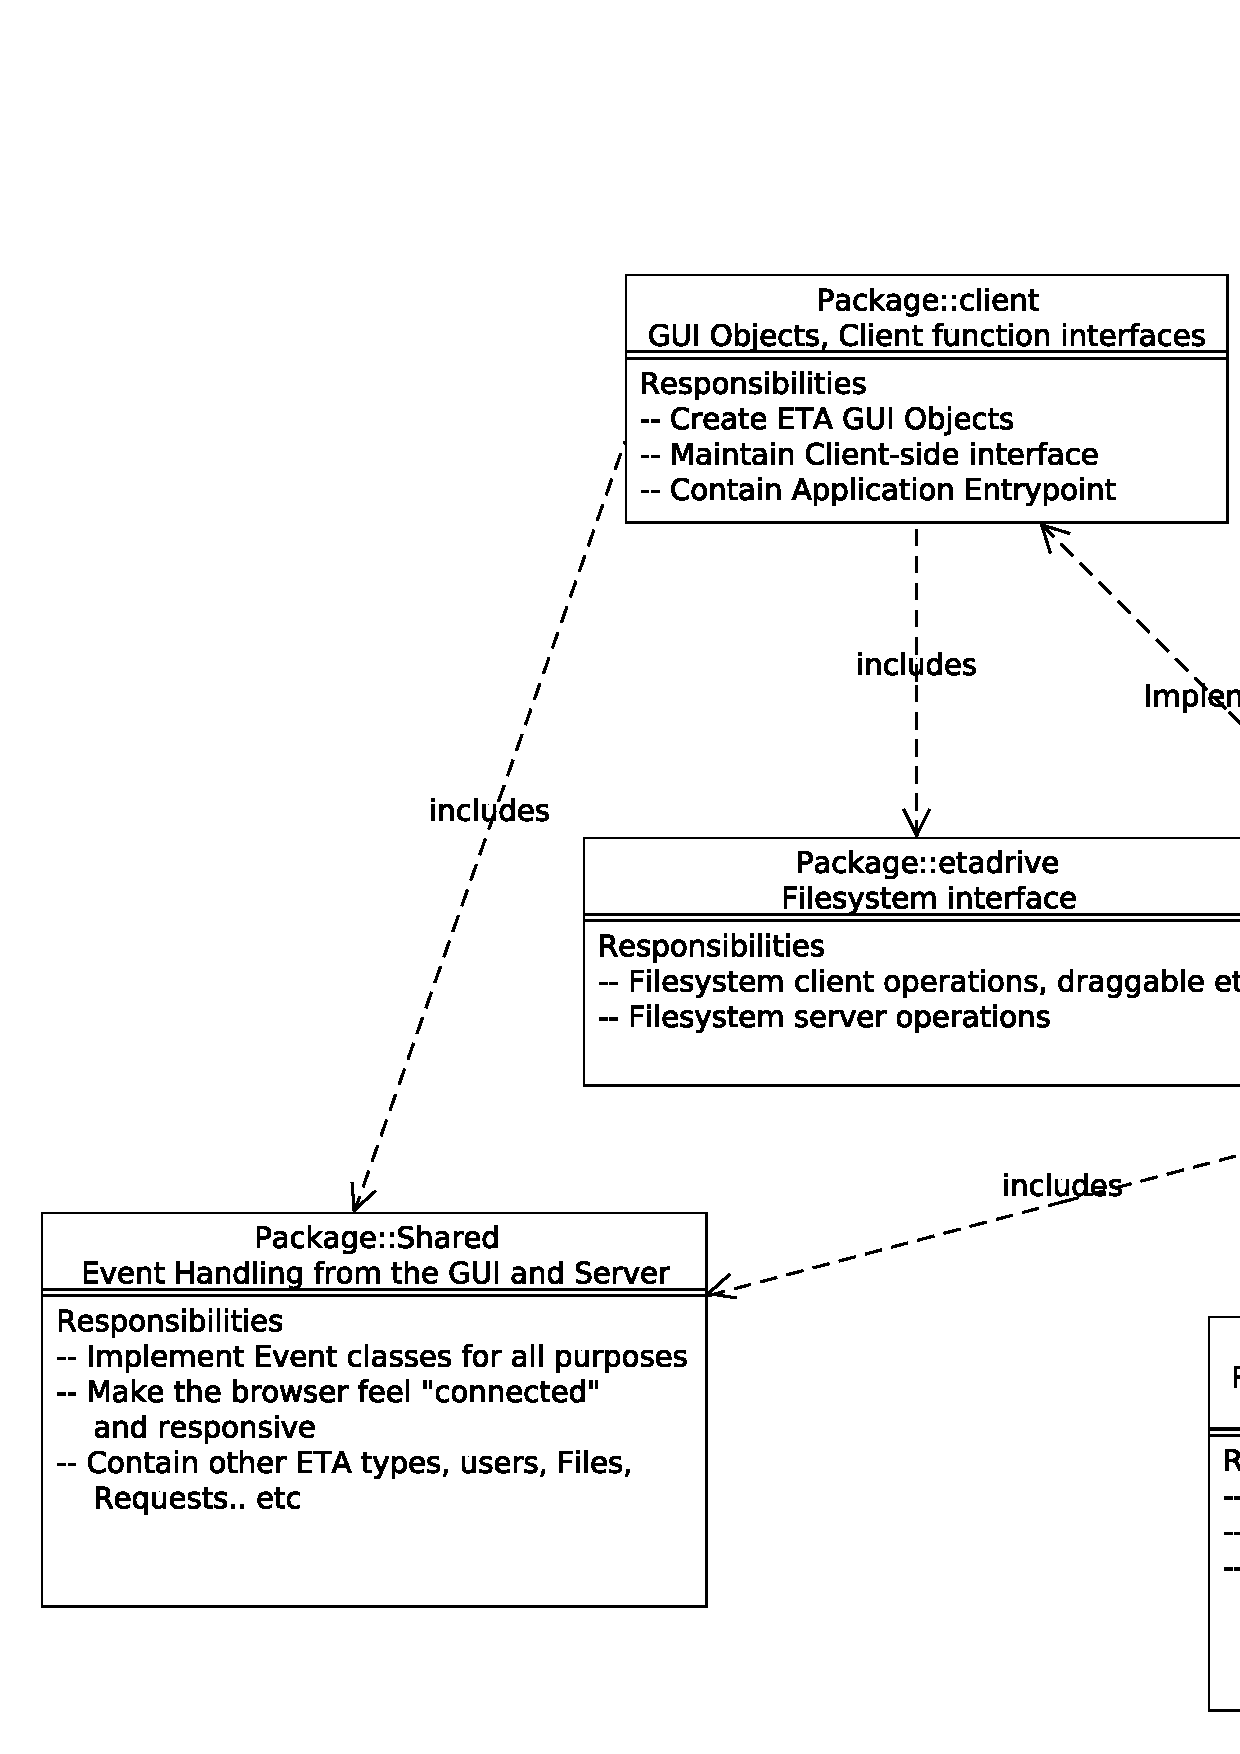
\includegraphics[width=1\textwidth]{ETAPackageOverview.jpg}
\caption{UML Diagram: ETA Package Overview}
\label{fig:ETAPackageOverview}
\end{figure}

\subsection{Dataflow}

 The way that ETA moves data is simple in concept, and complex in application. It is important to understand the different processes that belong to the Easy-Terminal-Alternative process group. These processes are, ETAStart, ETAMon, ETASubmit, and ETAUtil. Additionally, there are system services which ETA interacts, this is an authentication mechanism, a user manager, and a batch queue  for running jobs.
 
 When a user initially logs on, it first reaches the homepage of the web application. This is a HTML file which lives on the tomcat server. When a user logs into ETA, the server calls the authentication module, which then logs the user into the machine and executes ETAStart as that user. ETAStart is responsible for all of the interaction between the server and the user. It executes system calls, manages files, and submits jobs (Boyd). ETAStart is a persistent process and will not terminate unless explicitly told. 
 
 ETASubmit is the executable responsible for actually submitting the jobs to the batch system. ETASubmit is called from ETAStart, which will then finally call the monitoring process, ETAMon.
 
 ETAMon gets executed as the user anytime a job is submitted, it tracks the current progress of the job and notifies ETAStart when a job is finished. So when a user submits a job, ETAStart will call ETASubmit, which will then create an instance of ETAMon, which will then handle that job from start to finish.
 (Diagram needed) 
 \subsubsection{Job Submission}
 When a user first logs in, a token is created for that user in the database. This token will be used for authentication until their session has expired (ETA Source code). Upon authorization, a user can do several things, the most common being submitting a job. When a job is submitted, ETAStart executes the appropriate processes. An appropriate index is entered into the database representing the job. As long as this entry is active, the system will know the job is still running. ETAMon will handle the change of this value, which will then propagate it's way back to the end-user.
 
 The physical job will be run through the Sun Grid Engine Batch Scheduler. This is the scheduling and load balancing application for the CGRB cluster. Users may set several options, including total memory usage, estimated running time, number of execution threads, or even request a specific node to execute the job (Grid Entry Man Pages). Upon completion, the user will be notified and the standard output of the program will be displayed to the user. This information is stored in the users home directory under the folder ETA (ETA Source code). 

\subsubsection{Wrappers}
 The primary feature of Easy-Terminal-Alternative is to create wrappers, that is, web-driven forms that allow a user to interact with command line programs. When a user creates a wrapper, they choose a program from a list which is populated by ETAUtil. ETAUtil queries the server for a list of available applications (typically from the Linux /usr/bin folders). A user then inputs various fields which represent the different flags that are passed to the program. Upon completion, the wrapper is saved to the MySQL database.

 Each wrapper is associated with a user. These wrappers are typically private, but if marked as public (again stored in the database), any user may see and use the wrapper. When a job is submitted to ETASubmit, the command line arguments are parsed from the form built by the wrapper, and finally are placed into a string which will be submitted the Sun Grid Engine Batch scheduler.

\subsection{Runtime Environment}
Easy-Terminal-Alternative was designed to run on CentOS 6, and for the CGRB it is no different. Additionally, it requires a Batch scheduler, in this case The Sun Grid Engine. 


\setlength{\parindent}{0.5in}

\begin{workscited}

  \bibent
 Ambra Molesini, Alessandro Garcia, Christina von Flach Garcia Chavez, Thais Vasconcelos Batista, Stability assessment of aspect-oriented software architectures: A quantitative study, Journal of Systems and Software, Volume 83, Issue 5, May 2010, Pages 711-722, ISSN 0164-1212, 10.1016/j.jss.2009.05.022.
\\http://www.sciencedirect.com/science/article/pii/S0164121209001162. 

 \bibent
 "Apache Tomcat 6.0." \textit{Tomcat Documentation Index}. 9 Oct. 2012. Apache Foundation.  13 May 2013 http://tomcat.apache.org/tomcat-6.0-doc/. 
 
   \bibent
   Boyd, Alex. "Re: ETA Update" Message to the creator. 12 Dec. 2012. E-mail. An email with the original developer of Easy-Terminal-Alternative.
   
 \bibent
 Boyd, Alex. "Easy-Terminal-Alternative source code." Easy-Terminal-Alternative. Center for Genome Research and Biocomputing, 4, Sept. 2012. Web. 29, May 2013. 
\\https://www.github.com/cgrb/Easy-Terminal-Alternative. Source code to the actual application.

 \bibent
 "Google Web Toolkit." \textit{Developer's Guide}. 26 Oct. 2012. Google. 13 May 2013 \\https://developers.google.com/web-toolkit/doc/latest/DevGuide. 

 \bibent
 "Java Platform SE 7." \textit{Java Platform SE 7}. 28 July 2011. Oracle Inc. 13 May 2013 http://docs.oracle.com/javase/7/docs/api/. 


 \bibent
  Schroder, Carla. "Linux Bug \# 1: Bad Documentation" \textit{The Many Faces of Documentation}. N.p., 17 Nov. 2009. Web. 13 May 2013.\\ http://www.linuxplanet.com/linuxplanet/reports/6904/1/. 
  
  \bibent
  "Sun Grid Engine." \textit{Man Pages}. Apr. 2008. Web. 28 May 2013. \\ http://gridscheduler.sourceforge.net/htmlman/manuals.html.
  




 \end{workscited}
 \newpage
 \section{Primary Sources}
 \subsection{Email with Alex Boyd (creator)}
.\\
ETA Update\\
Steve Hill hillst@onid.orst.edu\\
12/10/12\\
\\
I see you have compiled most of the class files into different .jar files, ETAMon, ETAStart, ETAMonitor, ETASubmit, ETAUtil...
\\
Where does tomcat need them to execute at?
\\
I noticed all your shell scripts as well that initialize everything. Do they all get run at once? Or does tomcat just execute the bash scripts on startup?
\\
What services execute ETAStart and ETA itself (I assume the latter is tomcat).
\\
When you apply an update, do you just pull the files from git and recompile them into their .jar files?
\\\\
Thanks again,
\\
Steve
\\\\\\
RE: ETA Update\\
Alex Boyd alex@cgrb.oregonstate.edu\\
12/14/12
 \\\\
Ah sorry, I haven't had time to respond. I will set you up with everything you need to test on waterman tomorrow (Saturday) 
\\
ETAStart is the service that spawns off as each user, ETA will issue an su command and than spawn and detach itself from the proccess. THis is done when a user logins\\
ETAMon gets run everytime a job runs and tells ETA that it started/stopped etc\\
ETASubmit is a command line utitlty to submit jobs though ETA\\
ETAUtil is another comand line utility that will give you information about files like what program produced them etc..
\\\\
There is a settings file in WEB\-INF called settings that has all the settings for eta. one of them is ETA\_Path or something like that and it points to /local/cluster/ETA/dev and all the jar files are there as well as the .so library used for the login 
So I have a compile script that pulls the latest version from git and makes all the jars and compiles the webapp with GWT, this is actually done on a different server, I will give you more details tomorrow as well.

\end{document}